\chapter{Integración de componentes}\label{chapter:Integracion_de_componentes}

Para la construcción del robot se ha utilizado el kit de piezas Bioloid Premium de marca Robotis el cual incluye motores Dynamixel Ax-12+, una tarjeta controladora CM-510, un sensor Gyro, un manual, entre otros elementos. El manual incluye las instrucciones de como armar varios modelos de humanoide, el utilizado en este proyecto es el tipo B, haciendo uso de 16 motores. En la figura ~\ref{fig:frontal} y ~\ref{fig:trasera1} se puede observar la estructura del robot que aparece en el manual del kit. 

\begin{figure}[hbtp]
\centering
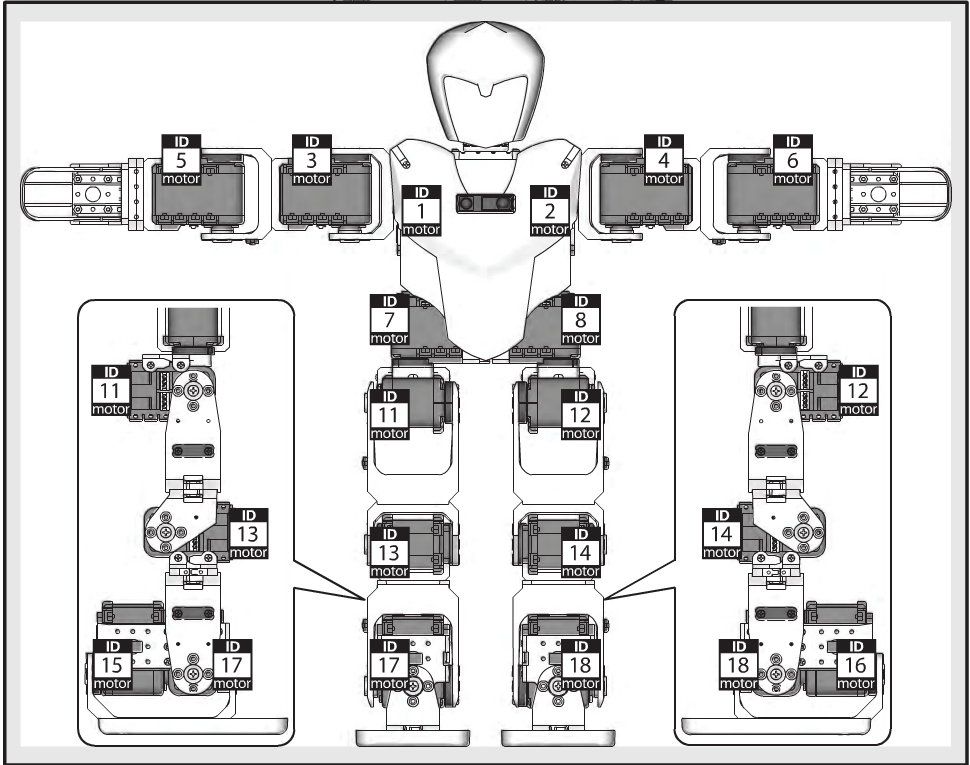
\includegraphics[scale=0.3]{imagenes/Robot.png}
\caption{vista frontal del robot. Se puede apreciar la identificación ‘ID’ de cada motor Dynamixel Ax-12+. Nota: los motores 9 y 10 no se utilizan}
\label{fig:frontal}
\end{figure}

\begin{figure}[hbtp]
\centering
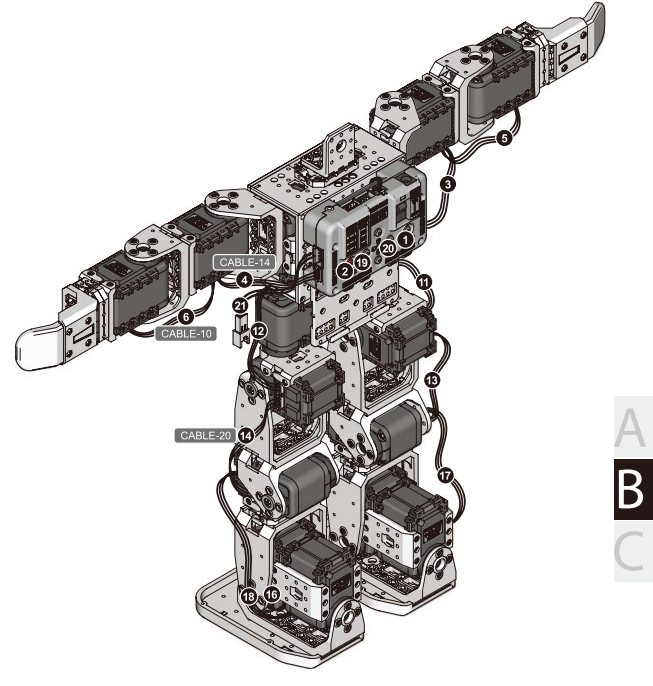
\includegraphics[scale=0.4]{imagenes/RobotTrasero.png}
\caption{Vista trasera del robot}
\label{fig:trasera1}
\end{figure}

En lugar de la utilización de la tarjeta CM-510 se ha decidido usar la tarjeta controladora Arbotix debido a que la controladora CM-510 no acepta la incorporación actuadores o dispositivos adicionales. La Arbotix permite la incorporación de nuevos actuadores y más dispositivos con sencillez. En la figura ~\ref{fig:trasera2} se puede observar la estructura del robot con la Arbotix incorporada. En la parte interna del tronco del robot se sitúa el sensor Gyro.

\begin{figure}[hbtp]
\centering
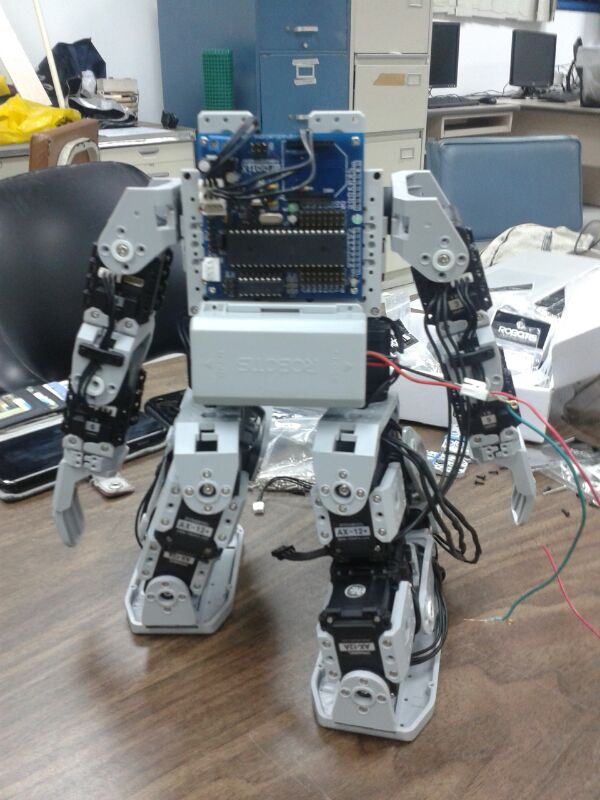
\includegraphics[scale=0.3]{imagenes/traseroDeJunny.jpg}
\caption{Vista trasera del robot con la Arbotix}
\label{fig:trasera2}
\end{figure}

\begin{figure}[hbtp]
\centering
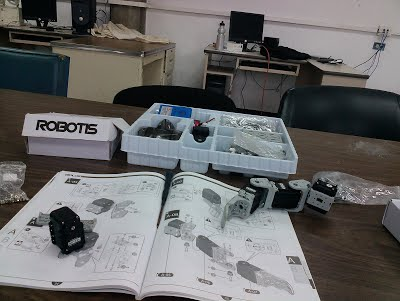
\includegraphics[scale=0.7]{imagenes/CIMG0225.jpg}
\caption{Manual de instrucciones y piezas del robot}
\end{figure}

Para el movimiento de la cámara se ha incorporado dos servomotores, uno para el movimiento horizontal y otro para el vertical. La conexión es pin a pin en los puertos especiales para ese tipo de motores (‘Hobby servos’) fuente (ver figura ~\ref{fig:puertosHobby}). La cámara ha sido conectada a la Raspberry Pi en el puerto CSI (ver la figura ~\ref{fig:camACSI}). El resultado de estas tres piezas instaladas en el robot se puede apreciar en la figura ~\ref{fig:servosycam}.

\begin{figure}[hbtp]
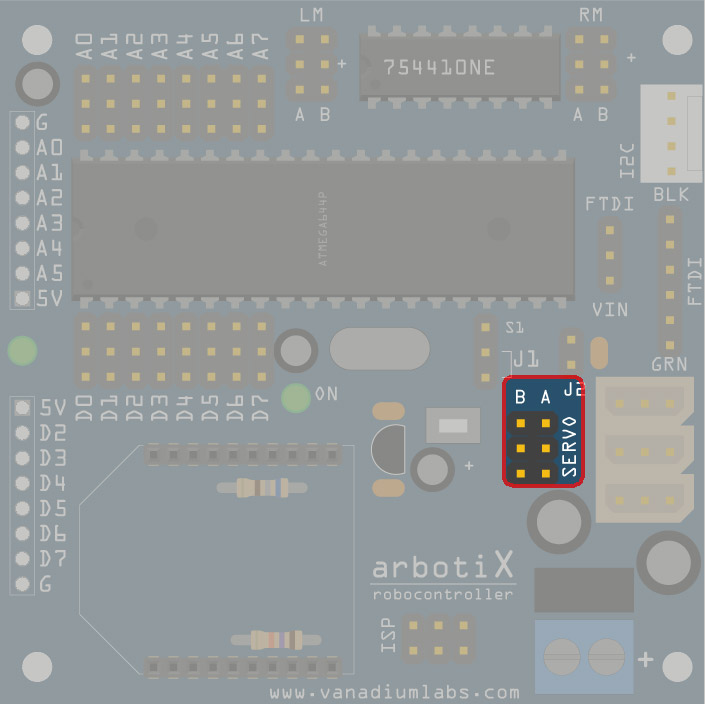
\includegraphics[scale=0.3]{imagenes/arbotix_hobby_servo.jpg}
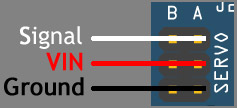
\includegraphics[scale=0.7]{imagenes/arbotix_hobbyservos_lines.jpg}
\caption{Ilustración de los puertos Hobby de la Arbotix}
\label{fig:puertosHobby}
\end{figure}

\begin{figure}[hbtp]
\centering
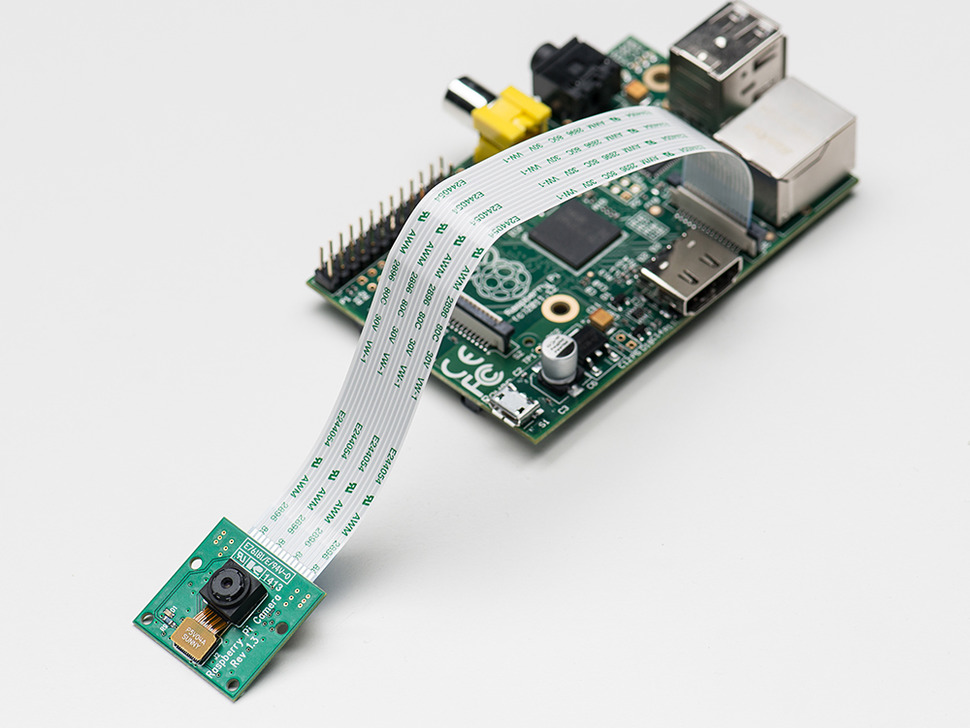
\includegraphics[scale=1]{imagenes/raspbCam.jpg}
\caption{Camara Raspberry Pi conectada al puerto CSI de la tarjeta}
\label{fig:camACSI}
\end{figure}
 
\begin{figure}[hbtp]
\centering
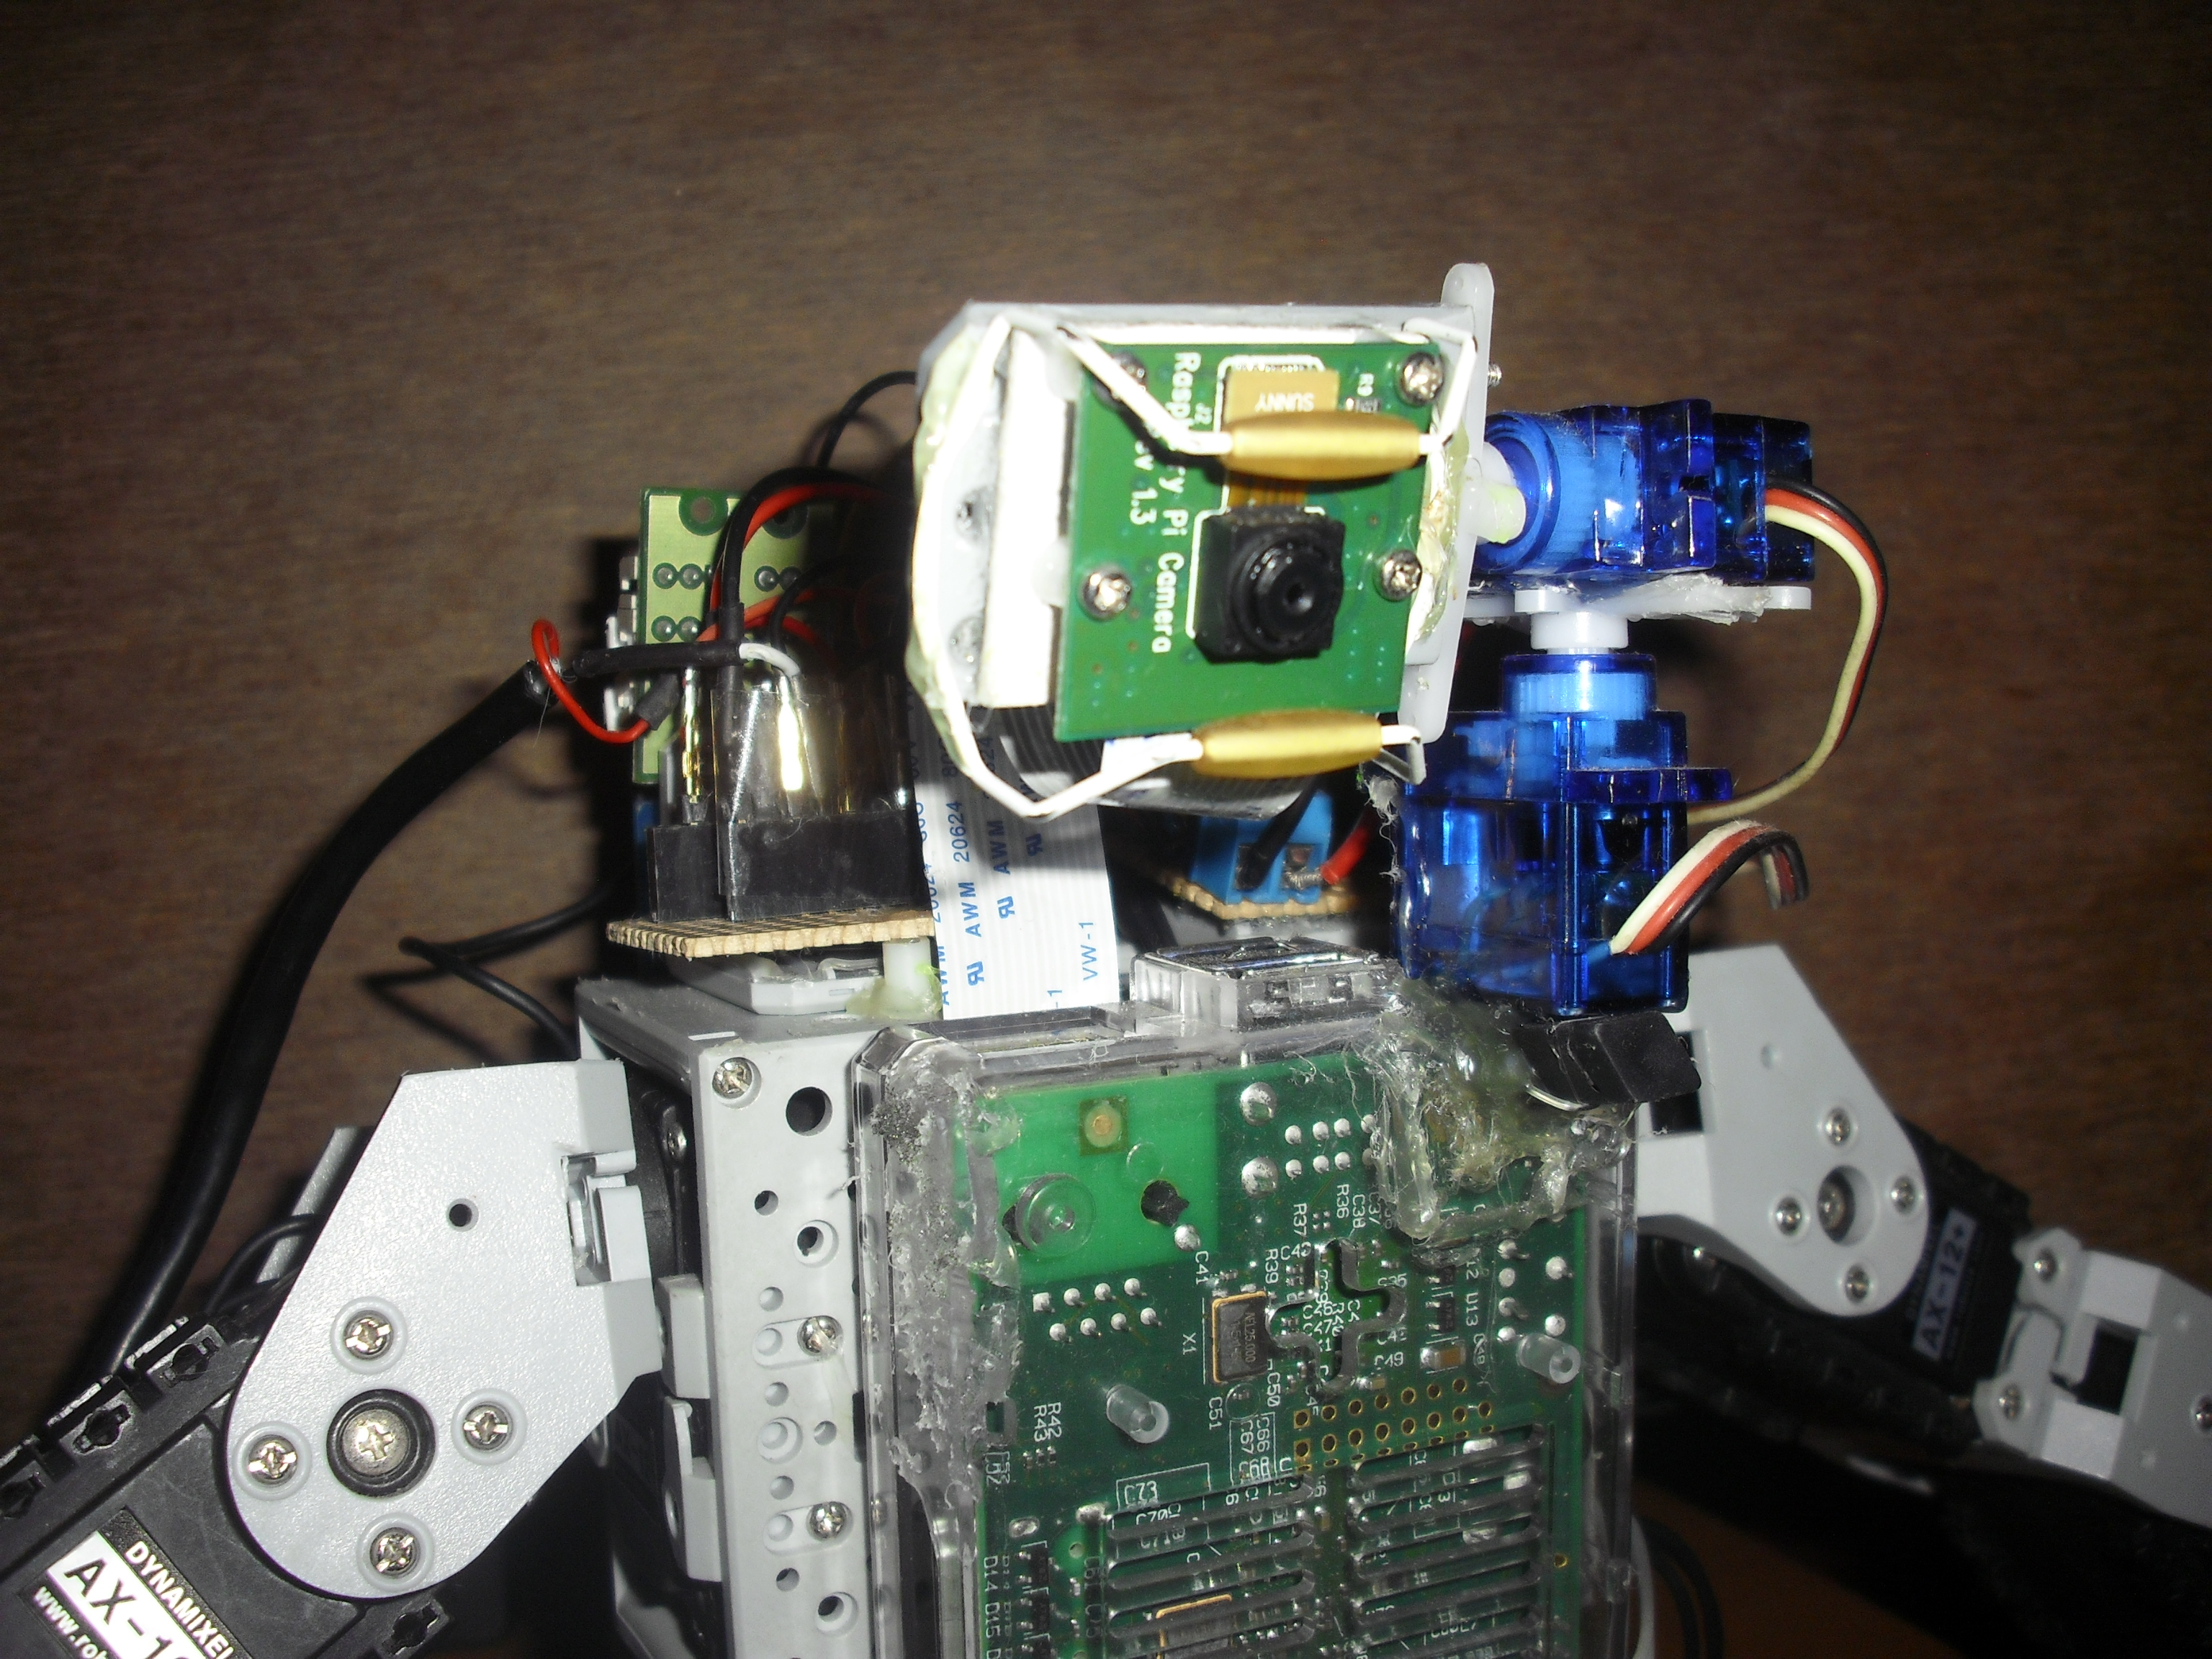
\includegraphics[scale=0.1]{imagenes/servosYcamara.JPG}
\caption{vista delantera del robot con la cámara y servomotores instalados}
\label{fig:servosycam}
\end{figure}

Los motores Dynamixel se conectan a la controladora Arbotix por medio de los puertos bioloid de la tarjeta. Sin embargo como la tarjeta solo cuenta con tres puertos y el robot posee cuatro extremidades, se ha optado por agregar un expansor de puertos bioloid y así conectar cada extremidad en un puerto diferente. La forma en la que se ha conectado estos motores se ejemplifica en 
la figura ~\ref{fig:arbotixConectados}. 

\begin{figure}[hbtp]
\centering
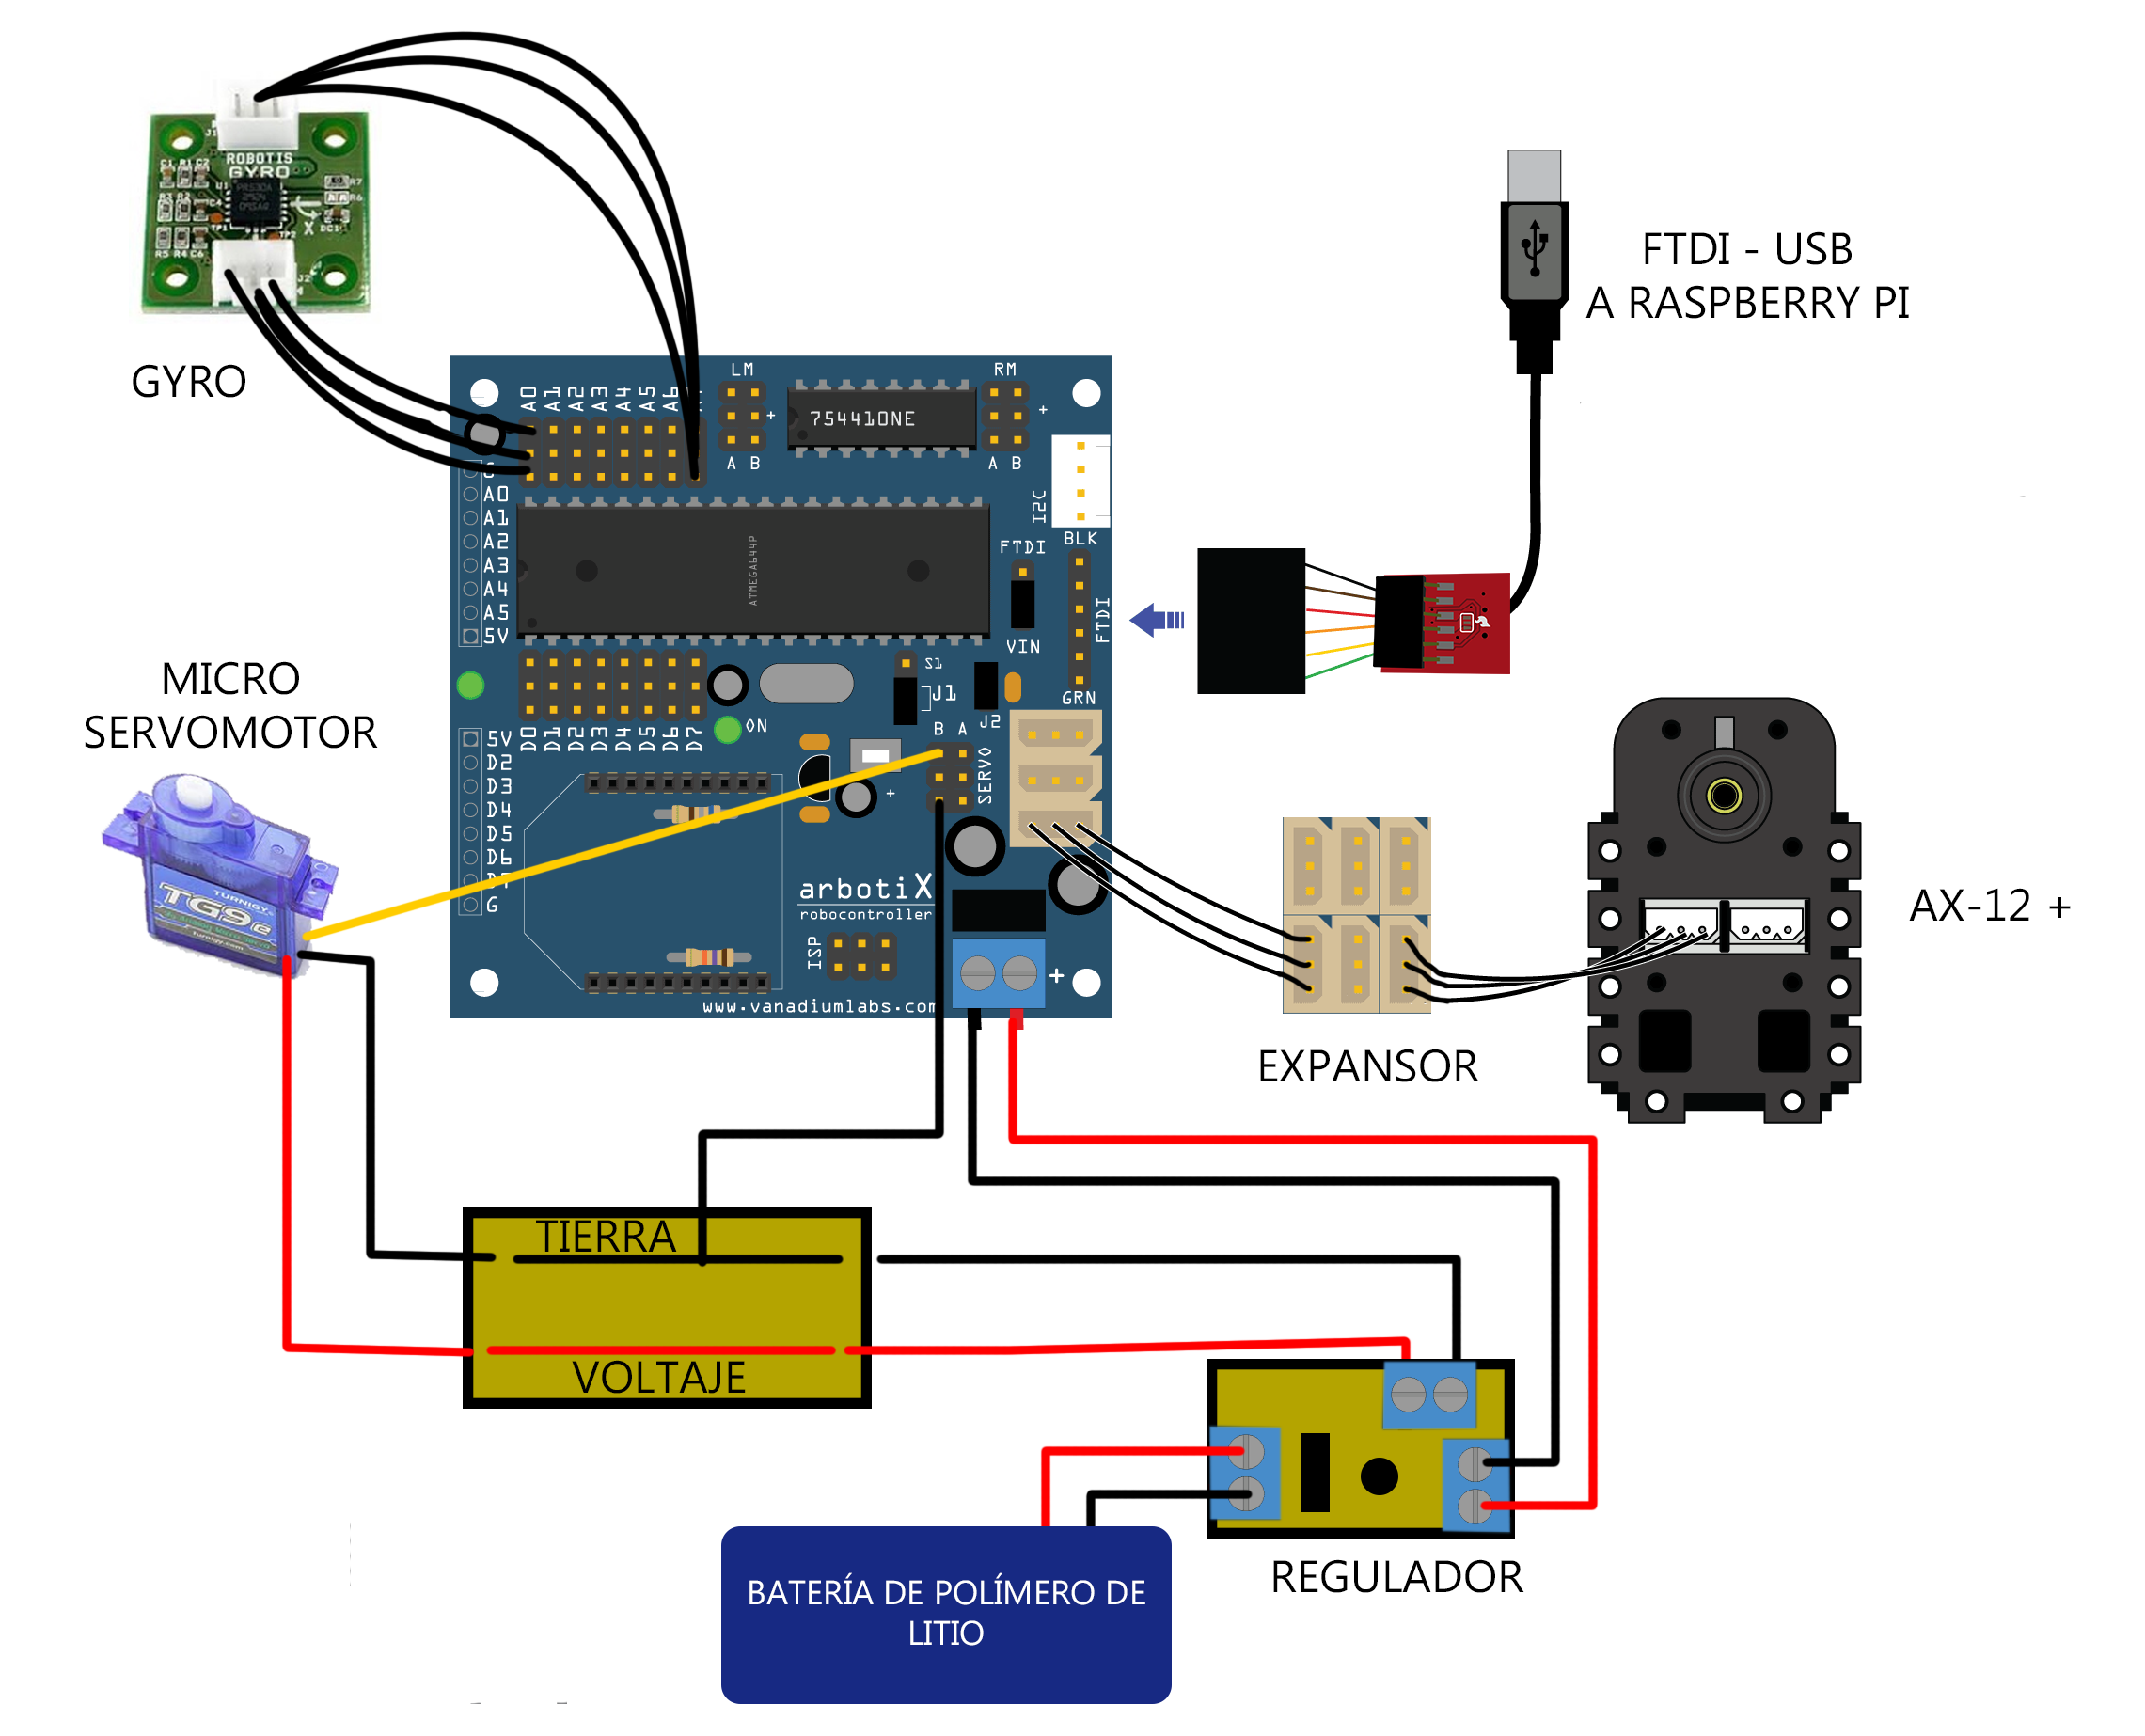
\includegraphics[scale=0.2]{imagenes/arbotix_servo.png}
\caption{Tarjeta controladora Arbotix y componentes conectados }
\label{fig:arbotixConectados}
\end{figure}

La comunicación de la tarjeta de Arbotix con la computadora, incluso con la Raspberry Pi, se realiza a través del puerto FTDI por medio un chip conectado como lo ilustra la figura ~\ref{fig:arbotixConectados}.

Como fuente de poder se ha utilizado una batería de polímero de litio de 11.1 V y 1 amp. Debido a que no todos los componentes poseen las mismas exigencias con respecto a voltaje y amperaje, se realizó un regulador (ver figura ~\ref{fig:circuito}) con  salida de 5 voltios para la tarjeta Raspberry Pi y los dos micro servomotores, y otra salida de 11.1 V para la tarjeta Arbotix que a su vez alimenta a los componentes conectados en ella (motores Dynamixel y Giroscopio).

\begin{figure}[hbtp]
\centering
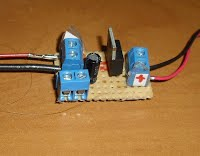
\includegraphics[scale=0.8]{imagenes/circuito.jpg}
\caption{Circuito con entrada de 11.1 V. Una salida de 5 V para los micro servomotores analogicos y tarjeta Raspberry Pi. Otra salida de 11 v para alimentar la controladora Arbotix.}
\label{fig:circuito}
\end{figure}

